\documentclass{article}\usepackage[]{graphicx}\usepackage[]{xcolor}
% maxwidth is the original width if it is less than linewidth
% otherwise use linewidth (to make sure the graphics do not exceed the margin)
\makeatletter
\def\maxwidth{ %
  \ifdim\Gin@nat@width>\linewidth
    \linewidth
  \else
    \Gin@nat@width
  \fi
}
\makeatother

\definecolor{fgcolor}{rgb}{0.345, 0.345, 0.345}
\newcommand{\hlnum}[1]{\textcolor[rgb]{0.686,0.059,0.569}{#1}}%
\newcommand{\hlstr}[1]{\textcolor[rgb]{0.192,0.494,0.8}{#1}}%
\newcommand{\hlcom}[1]{\textcolor[rgb]{0.678,0.584,0.686}{\textit{#1}}}%
\newcommand{\hlopt}[1]{\textcolor[rgb]{0,0,0}{#1}}%
\newcommand{\hlstd}[1]{\textcolor[rgb]{0.345,0.345,0.345}{#1}}%
\newcommand{\hlkwa}[1]{\textcolor[rgb]{0.161,0.373,0.58}{\textbf{#1}}}%
\newcommand{\hlkwb}[1]{\textcolor[rgb]{0.69,0.353,0.396}{#1}}%
\newcommand{\hlkwc}[1]{\textcolor[rgb]{0.333,0.667,0.333}{#1}}%
\newcommand{\hlkwd}[1]{\textcolor[rgb]{0.737,0.353,0.396}{\textbf{#1}}}%
\let\hlipl\hlkwb

\usepackage{framed}
\makeatletter
\newenvironment{kframe}{%
 \def\at@end@of@kframe{}%
 \ifinner\ifhmode%
  \def\at@end@of@kframe{\end{minipage}}%
  \begin{minipage}{\columnwidth}%
 \fi\fi%
 \def\FrameCommand##1{\hskip\@totalleftmargin \hskip-\fboxsep
 \colorbox{shadecolor}{##1}\hskip-\fboxsep
     % There is no \\@totalrightmargin, so:
     \hskip-\linewidth \hskip-\@totalleftmargin \hskip\columnwidth}%
 \MakeFramed {\advance\hsize-\width
   \@totalleftmargin\z@ \linewidth\hsize
   \@setminipage}}%
 {\par\unskip\endMakeFramed%
 \at@end@of@kframe}
\makeatother

\definecolor{shadecolor}{rgb}{.97, .97, .97}
\definecolor{messagecolor}{rgb}{0, 0, 0}
\definecolor{warningcolor}{rgb}{1, 0, 1}
\definecolor{errorcolor}{rgb}{1, 0, 0}
\newenvironment{knitrout}{}{} % an empty environment to be redefined in TeX

\usepackage{alltt}

\usepackage{amsmath}
\usepackage[vmargin=3cm, hmargin=2cm, headheight=14pt]{geometry}
\usepackage[font=sf, labelfont={sf}, margin=1cm]{caption}
\usepackage{placeins}
\usepackage{hyperref}
\IfFileExists{upquote.sty}{\usepackage{upquote}}{}
\begin{document}



% =============================================================================
\section{The Model} \label{sec:Model}
% =============================================================================

The marginal distributions are of the form: $$y_{g,s}\sim NBin(\mu_{g,s}, \sigma_{g,s}),$$ with $$log(\mu_{g,s})=log(nc_{s} \times \boldsymbol{w_{s}^T} \times \boldsymbol{m_{g}} \times sd_{s}) + gd_{g} + se_{s,g}$$ and $$log(\sigma_{g,s})=\alpha_{g}+\beta_{g}\times log(nc_{s} \times \boldsymbol{w_{s}^T} \times \boldsymbol{m_{g}} \times sd_{s}).$$ The expression $y$ of gene $g$ in spot $s$, $y_{g,s}$, depends on the level of the mean $\mu_{g,s}$ on $nc_{s}$, the number of cells in spot $s$, $\boldsymbol{w_{s}^T}$, the cell type proportions of spot $s$, $\boldsymbol{m_{g}}$, the mean contributions of the cell types to the expression of gene $g$, $sd_{s}$, a spot detection efficiency for the experiment, $gd_{g}$, a (log) gene detection efficiency for the experiment, and $se_{s,g}$ the (log) spatial effect of spot $s$ on the expression of gene $g$. The term $nc_{s} \times \boldsymbol{w_{s}^T} \times \boldsymbol{m_{g}}$ can be thought of as a theoretical mean, without taking into account technical errors in the experiment and a spatial effect on gene expressions beyond that which is due to spatial distribution of the cell types. The technical errors eluded to above are encompassed in $sd_{s}$ and $gd_{g}$. The marginal distributions are combined to spot level distributions with a Gaussian copula. For more details see the actual master thesis.


% =============================================================================
\section{Some distributions of estimated parameters for the mouse kidney dataset} \label{sec:distributions_estimation}
% =============================================================================



The estimated number of cells per spot can be inspected in figure~\ref{f:ncells_mkc}. Towards the middle of the sample the estimated
number of cells are higher. The spot detection efficiencies (figure~\ref{f:sde_mkc}) have no spatial structure which is in accordance with the assumptions of the model.

\begin{figure}[h]
\begin{minipage}[c]{0.5\textwidth}
\begin{knitrout}
\definecolor{shadecolor}{rgb}{0.969, 0.969, 0.969}\color{fgcolor}

{\centering 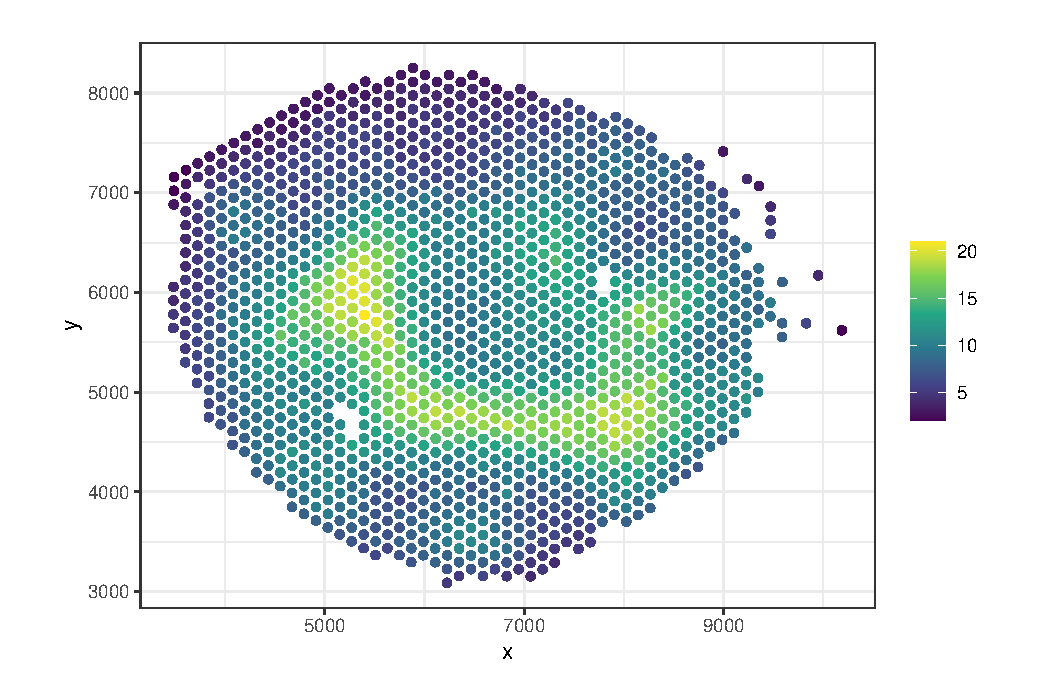
\includegraphics[width=\maxwidth]{plots/pc7-1} 

}


\end{knitrout}
  \caption{Estimated number of cells per spot for the mouse kidney ST data}
\label{f:ncells_mkc}
\end{minipage}
\hfill
\begin{minipage}[c]{0.5\textwidth}
\begin{knitrout}
\definecolor{shadecolor}{rgb}{0.969, 0.969, 0.969}\color{fgcolor}

{\centering 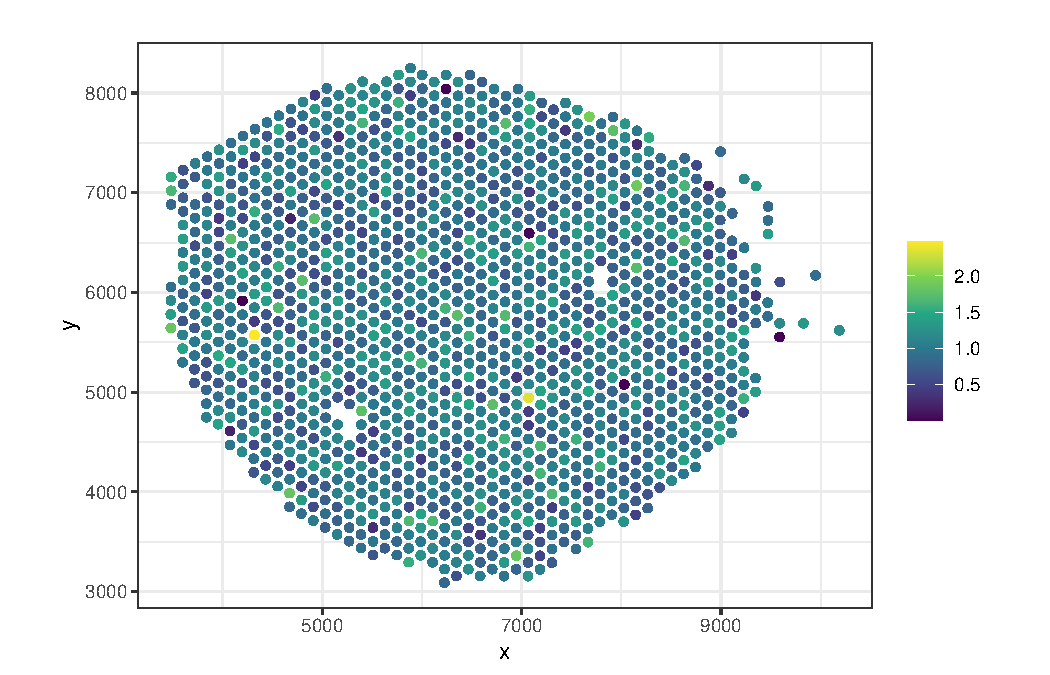
\includegraphics[width=\maxwidth]{plots/pc8-1} 

}


\end{knitrout}
  \caption{Estimated spot detection efficiencies for the mouse kidney ST data}
\label{f:sde_mkc}
\end{minipage}
\end{figure}

For the two genes Kap and Gpx3 the domain effects on the mean of their expressions are shwon in figure~\ref{f:re_mkc_Kap} for gene Kap and figure~\ref{f:re_mkc_Gpx3} for gene Gpx3. The domain effects are set to give a geometric mean of 1.

\begin{figure}[h]
\begin{minipage}[c]{0.5\textwidth}
\begin{knitrout}
\definecolor{shadecolor}{rgb}{0.969, 0.969, 0.969}\color{fgcolor}

{\centering 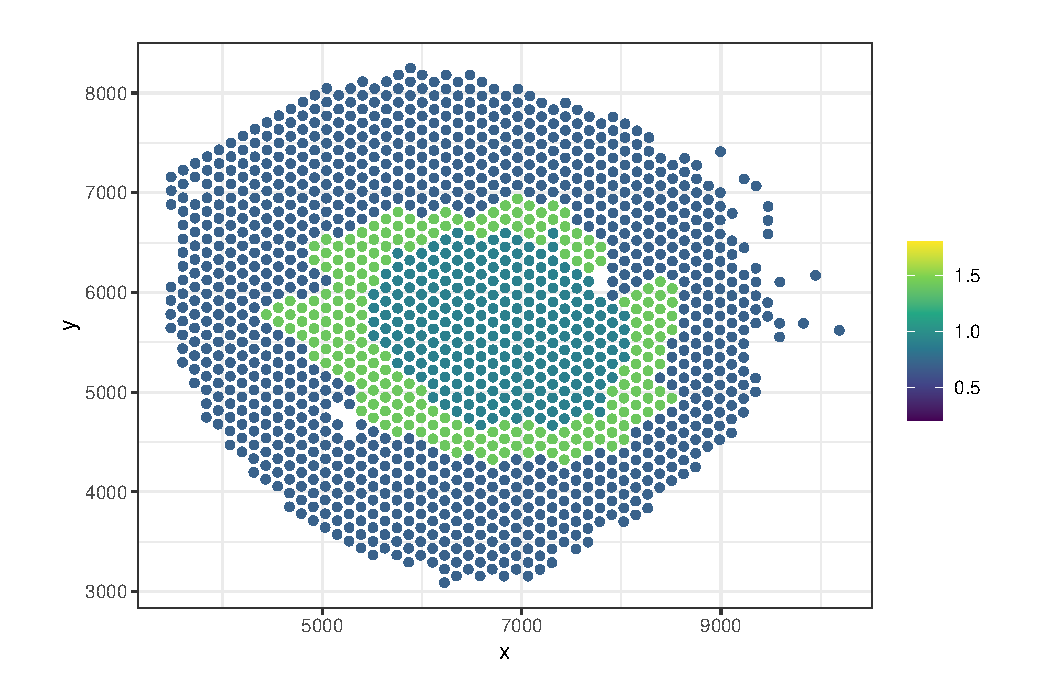
\includegraphics[width=\maxwidth]{plots/pc9-1} 

}


\end{knitrout}
  \caption{Domain effects of gene Kap for the DLPFC ST data}
\label{f:re_mkc_Kap}
\end{minipage}
\hfill
\begin{minipage}[c]{0.5\textwidth}
\begin{knitrout}
\definecolor{shadecolor}{rgb}{0.969, 0.969, 0.969}\color{fgcolor}

{\centering 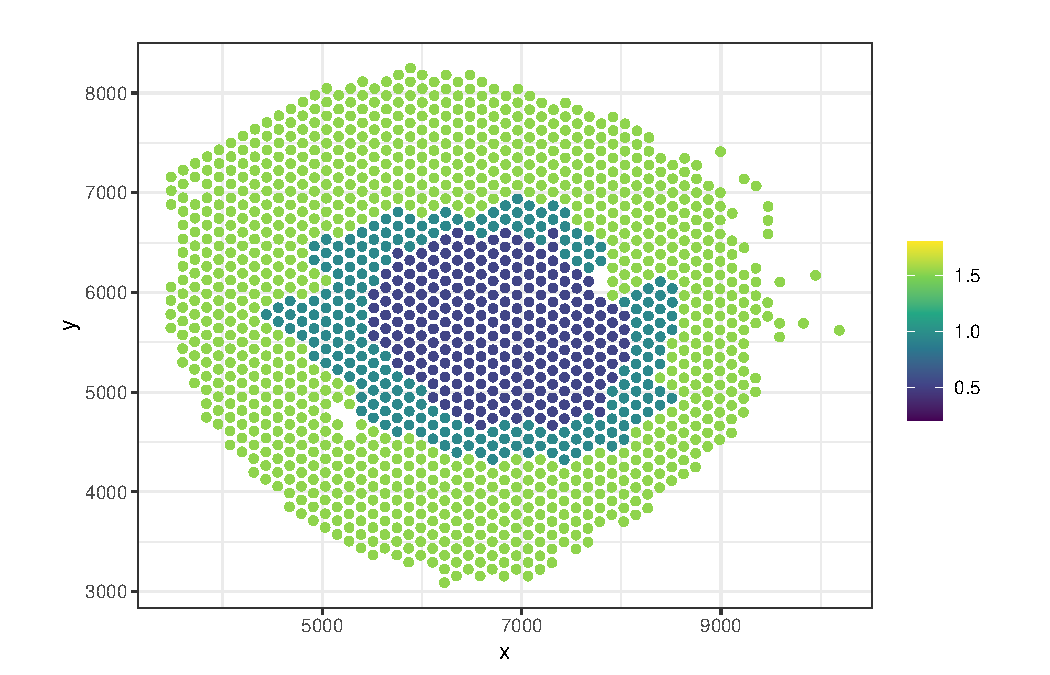
\includegraphics[width=\maxwidth]{plots/pc10-1} 

}


\end{knitrout}
  \caption{Domain effects of gene Gpx3 for the DLPFC ST data}
\label{f:re_mkc_Gpx3}
\end{minipage}
\end{figure}



Fitted means and standard deviations per spot for gene Tmsb4x can be found in figure~\ref{f:mean_mkc_Tmsb4x} and figure~\ref{f:sd_mkc_Tmsb4x}.

\begin{figure}[h]
\begin{minipage}[c]{0.5\textwidth}
\begin{knitrout}
\definecolor{shadecolor}{rgb}{0.969, 0.969, 0.969}\color{fgcolor}

{\centering 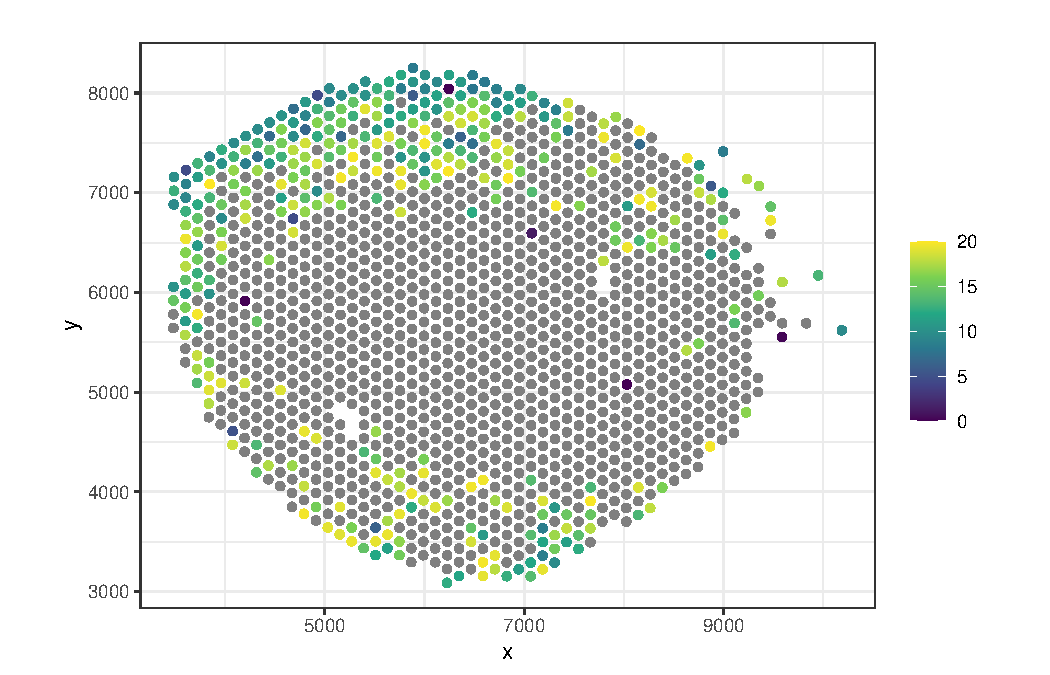
\includegraphics[width=\maxwidth]{plots/pc14-1} 

}


\end{knitrout}
  \caption{Fitted mean of gene Tmsb4x for the DLPFC ST data}
\label{f:mean_mkc_Tmsb4x}
\end{minipage}
\hfill
\begin{minipage}[c]{0.5\textwidth}
\begin{knitrout}
\definecolor{shadecolor}{rgb}{0.969, 0.969, 0.969}\color{fgcolor}

{\centering 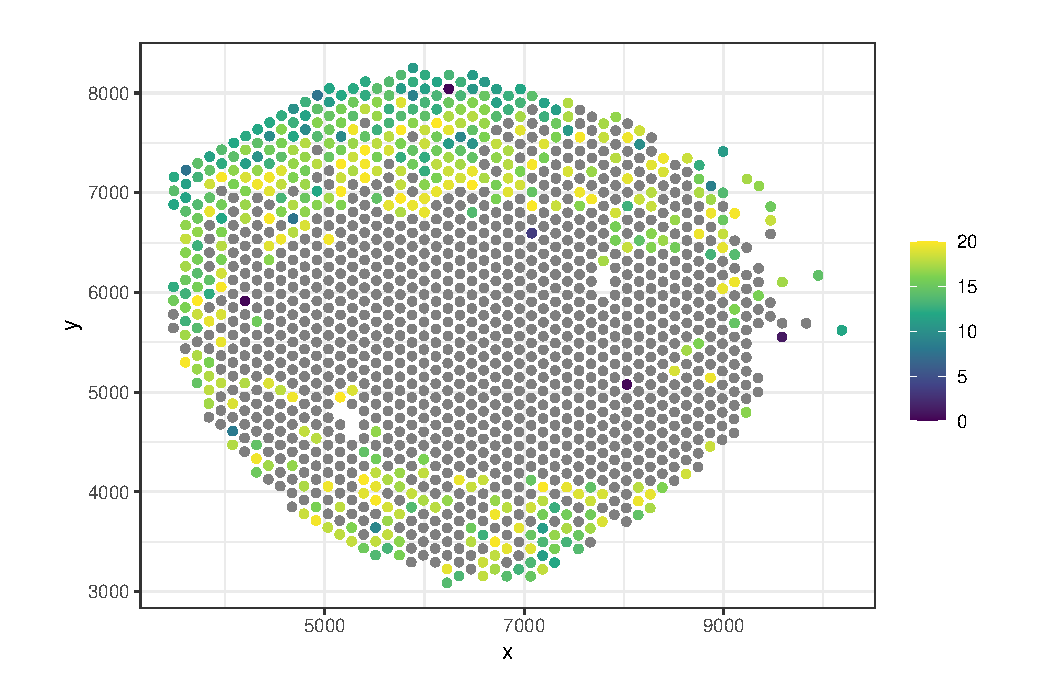
\includegraphics[width=\maxwidth]{plots/pc15-1} 

}


\end{knitrout}
  \caption{Fitted standard deviation of gene Kap for the DLPFC ST data}
\label{f:sd_mkc_Tmsb4x}
\end{minipage}
\end{figure}

Figure~\ref{f:hist_gde_mkc} shows estimated gene detection efficiencies for the mouse kidney dataset. These are mostly near zero, because the spot detection were set to be near 1 and the generally low efficiency of the VISIUM platform on which the spatial transcriptomic data was gathered compared to single cell RNA sequencing technologies.

\begin{figure}[h]
\centering
\scalebox{.8}{
\begin{knitrout}
\definecolor{shadecolor}{rgb}{0.969, 0.969, 0.969}\color{fgcolor}

{\centering 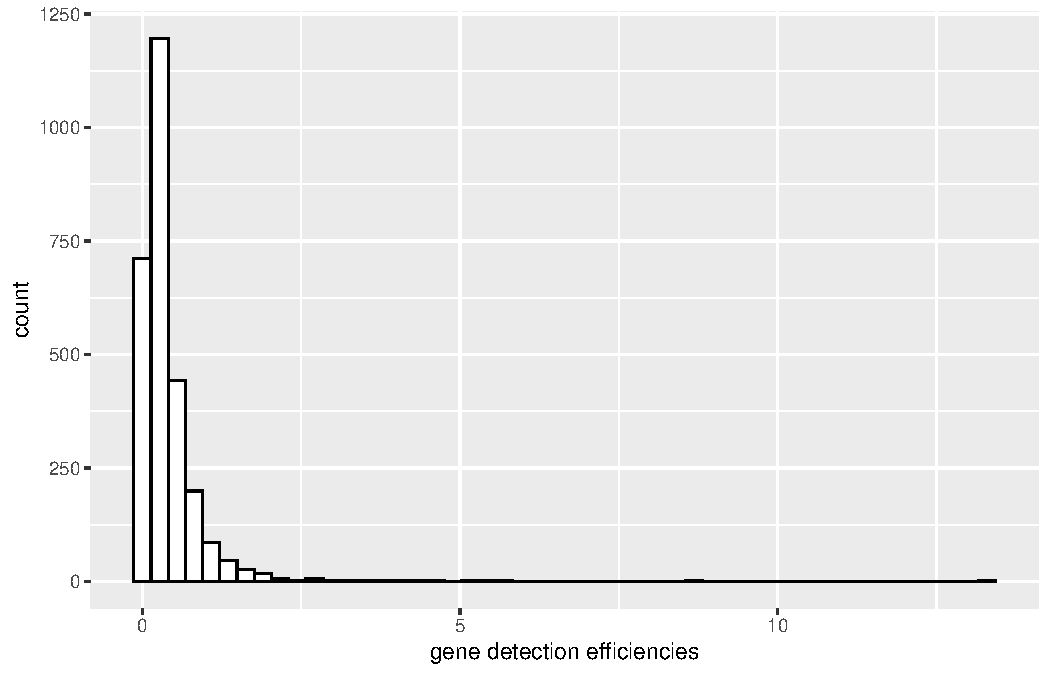
\includegraphics[width=\maxwidth]{plots/pc16-1} 

}


\end{knitrout}
}
\caption{Histogram of the gene detection efficiecnies for the mouse kidney data. Most of the genes have a low estimated detection efficiency.}
\label{f:hist_gde_mkc}
\end{figure}

\FloatBarrier
\newpage

% =============================================================================
\section{Some plots to evaluate the simulate data} \label{sec:evaluate_simulation}
% =============================================================================



Gene-wise means and standard deviations are well preserved in the simulated data (figure~\ref{f:gwm_sim_true} and figure~\ref{f:gwsd_sim_true}). The spot-wise means and standard deviations are less well preserved, because the marginal expressions were fit for genes, not for spots (figure~\ref{f:gwsd_sim_true} and figure~\ref{f:spot_sd_sim_true}). 

\begin{figure}[h]
\centering
\scalebox{.8}{
\begin{knitrout}
\definecolor{shadecolor}{rgb}{0.969, 0.969, 0.969}\color{fgcolor}

{\centering 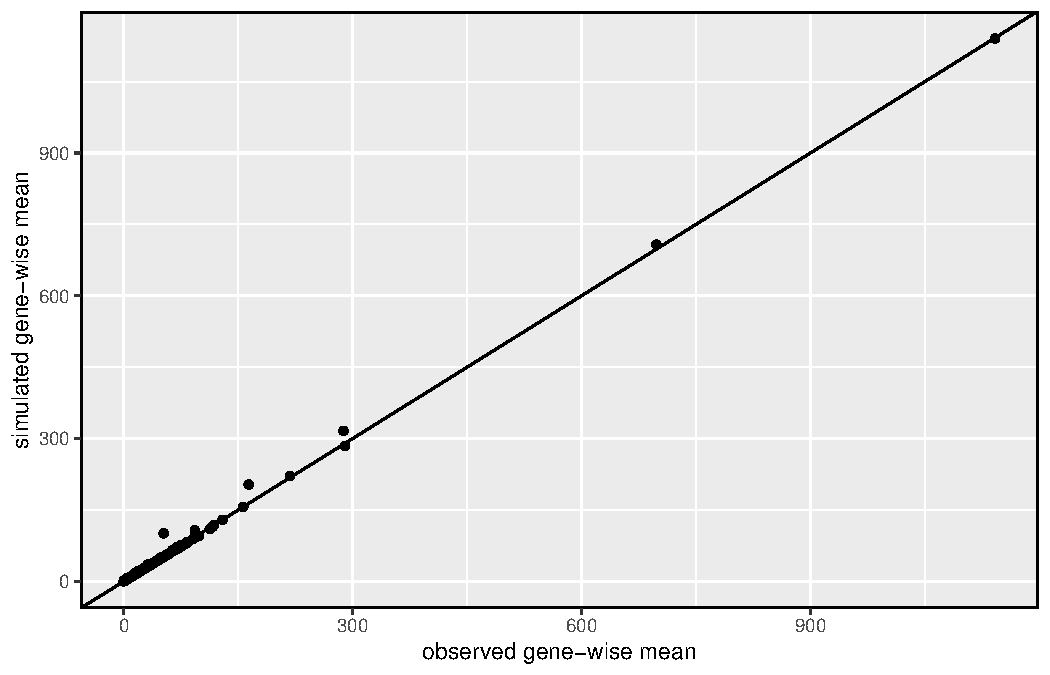
\includegraphics[width=\maxwidth]{plots/pc18-1} 

}


\end{knitrout}
}
\caption{Gene-wise means of observed vs simulated data. The means are preserved in the simulated data.}
\label{f:gwm_sim_true}
\end{figure}

\begin{figure}[h]
\centering
\scalebox{.8}{
\begin{knitrout}
\definecolor{shadecolor}{rgb}{0.969, 0.969, 0.969}\color{fgcolor}

{\centering 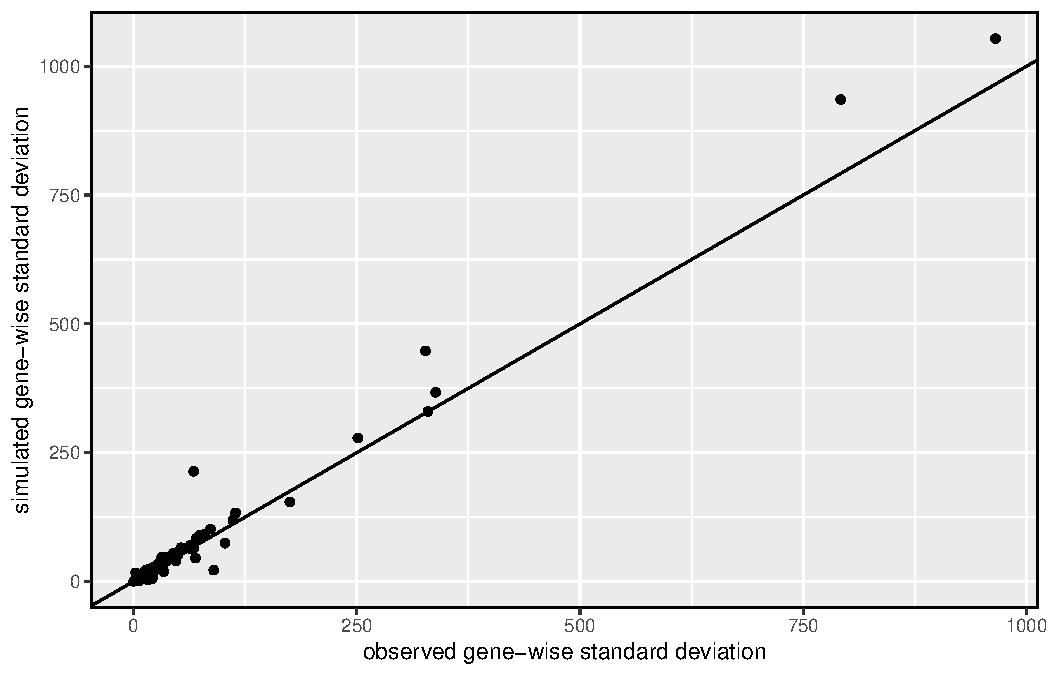
\includegraphics[width=\maxwidth]{plots/pc19-1} 

}


\end{knitrout}
}
\caption{Gene-wise standard deviations of observed vs simulated data. For most genes, the standard devations are similar, but there are outliers for which the standard deviation in the observed data is very low, whereas it is high in the simulated data.}
\label{f:gwsd_sim_true}
\end{figure}

\begin{figure}[h]
\centering
\scalebox{.8}{
\begin{knitrout}
\definecolor{shadecolor}{rgb}{0.969, 0.969, 0.969}\color{fgcolor}

{\centering 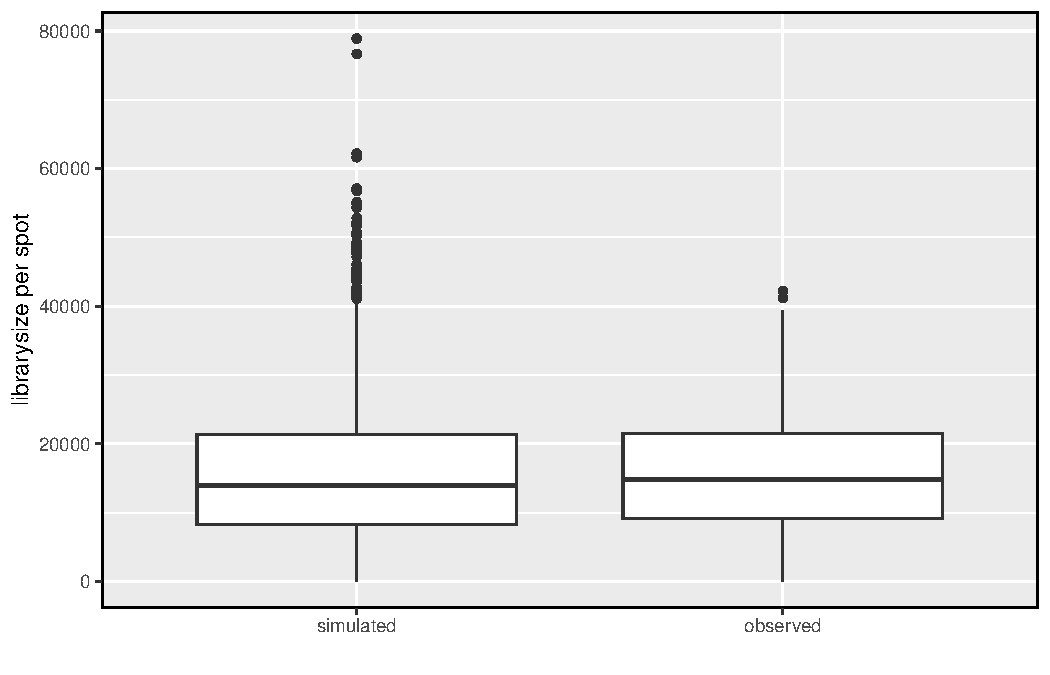
\includegraphics[width=\maxwidth]{plots/pc24-1} 

}


\end{knitrout}
}
\caption{Observed vs simulated librarysizes per spot. The distribution of librarysizes per spots stays roughly the same in the simulated data.}
\label{f:spot_libsize_sim_true}
\end{figure}

\begin{figure}[h]
\centering
\scalebox{.8}{
\begin{knitrout}
\definecolor{shadecolor}{rgb}{0.969, 0.969, 0.969}\color{fgcolor}

{\centering 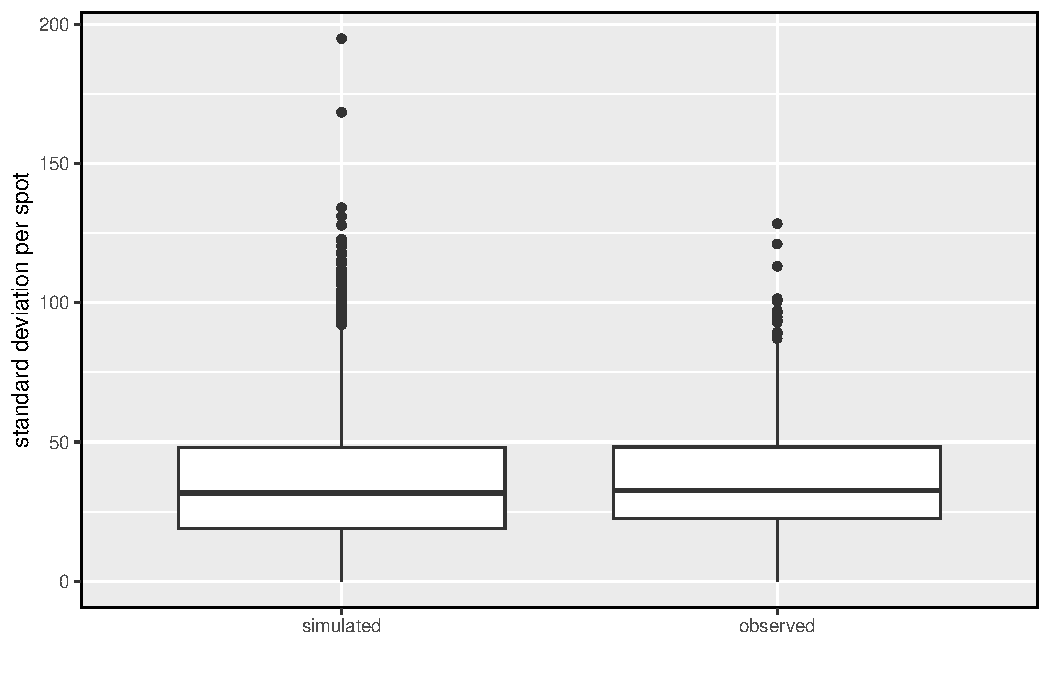
\includegraphics[width=\maxwidth]{plots/pc25-1} 

}


\end{knitrout}
}
\caption{Observed vs simulated standard devations of expressions per spot. The distribution of standard deviations per spots stays roughly the same in the simulated data.}
\label{f:spot_sd_sim_true}
\end{figure}

\end{document}
